\section{Software}
Die Steuerung der Segel soll durch zwei verteilte Systeme erfolgen, die über eine Ethernet-Verbindung miteinander kommunizieren. Die Idee dahinter ist, die Berechnungen für die Ausrichtung der Segel in Abhängigkeit der Windstärke und -Richtung (Controllino) von der hardwarenahen Verarbeitung der Sensoren und Aktuatoren (stm32) logisch zu trennen. \\
Die vorliegende Arbeit konzentriert sich dabei lediglich auf das System der Sensoren und Aktuatoren, welches mit dem stm32 realisiert wurde. Die Aufgabe dieses Systems ist, zunächst die Linearführung zu kalibrieren, damit die aktuelle Position korrekt ermittelt werden kann. Außerdem soll über die Buttons am Gehäuse und zusätzlich über einen Webserver eine manuelle Steuerung ermöglicht werden. Während des Automatikbetriebs geschieht ein regelmäßiger Austausch aller relevanter Daten über eine REST basierte Schnittstelle. Dies beinhaltet u.A. die Information über aktuelle Windbedingung, Position der Segel, eventuelle Fehlerzustände (z.B. Motorfehler oder Überstrom) und daraus resultierende Befehle zur Anpassung der Segelstellung.
Für die Implementierung wurde die Software in komponentenorientierte Module eingeteilt:

\begin{figure}[h]
	\centering
	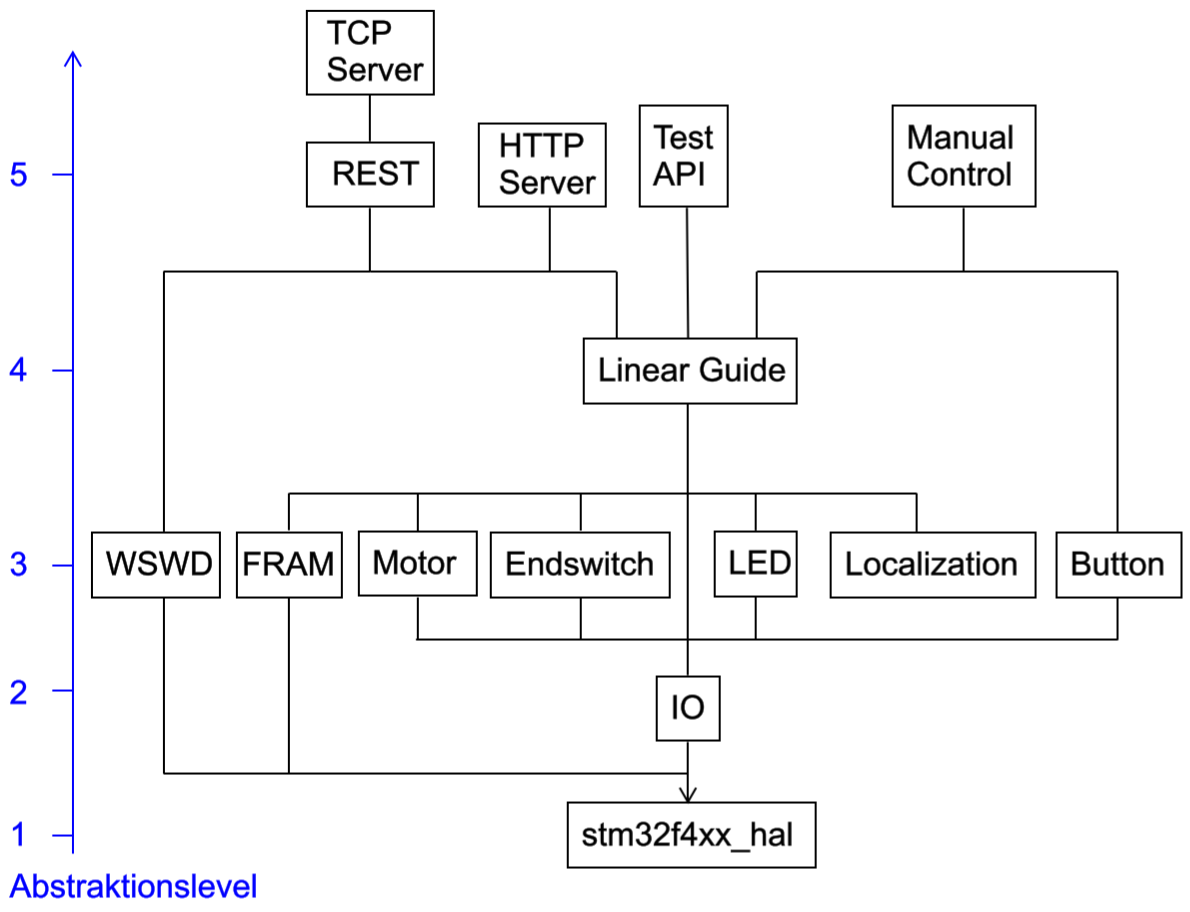
\includegraphics[width=0.6\linewidth]{images/Software/Modulestructure.png}
	\caption{Software Modulstruktur}
	\label{fig:modulestructure}
\end{figure}
\noindent
Abbildung \ref{fig:modulestructure} zeigt abwärtsgerichtet, wie die einzelnen Module aufeinander zugreifen. Auf unterster Abstraktionsebene laufen jegliche Operationen über die Standardbibliothek des Mikrocontrollers \texttt{stm32f4xx\_hal}. Darüber liefert das \texttt{IO}-Modul ein Set aus Hilfsfunktionen und -Strukturen für den allgemeinen Zugriff auf die GPIO-Pins und zum Auslesen analoger Messwerte der einzelnen Sensoren. Ebene drei umfasst hauptsächlich Module, welche alle relevanten Funktionalitäten der physischen Teilkomponenten des Systems implementieren, wie z.B. das Anemometer \texttt{WSWD} oder der \texttt{Motor}. Einige davon greifen dabei auf das \texttt{IO}-Modul zu, wobei der allgemeine GPIO-Zugriff von einer spezifischen Funktion eingekapselt wird, wie z.B. das Einschalten einer LED im Falle des \texttt{LED-Moduls}. Eine Ausnahme ist das \texttt{Localization}-Modul, welches keine physische Komponente darstellt, sondern einige Hilfsfunktionen zur Kalibrierung und Positionsberechnung bereitstellt. Während die Module bis Ebene drei überwiegend allgemeingültig entworfen sind, enthält das \texttt{Linear Guide}-Modul anwendungsspezifische Funktionen. Als zentrales Element bildet dieses ein High-Level Interface zur Verwendung der Teilkomponenten \texttt{FRAM}, \texttt{Motor}, \texttt{Endswitch}, \texttt{LED}, \texttt{Localization} und \texttt{IO}. Die Module der obersten Abstraktionsebene bilden die direkten Schnittstellen zur Außenwelt. Das \texttt{Manual Control}-Modul ermöglicht die manuelle Steuerung der Linearführung über die User-Buttons am Gehäuse und insbesondere die Umsetzung des Kalibrierungsprozesses. Auf der anderen Seite kann das System auch durch einen HTTP Webserver überwacht und gesteuert werden. Außerdem werden im \texttt{REST}-Modul die Anfragen des Controllinos über die \texttt{TCP Server}-Verbindung verarbeitet, wie bereits oben erwähnt. Zuletzt wurde ein \texttt{Test}-Modul implementiert, dass die Funktionalitäten der Module auf Ebene drei verifiziert. Dazu wurde ein einfaches Batch-Skript geschrieben, das die einzelnen Testcases auflistet und die Auswahl über UART an den  Mikrocontroller sendet, sodass im \texttt{Test}-Modul eine entsprechende Funktion ausgeführt wird.\\In den nachfolgenden Abschnitten wird genauer auf die einzelnen Module eingegangen, beginnend mit dem untersten Abstraktionslevel.

\subsection{IO}
Dieses Modul soll den lesenden und schreibenden Zugriff auf jegliche GPIO-Pins erleichtern, die zur Kontrolle jeglicher Steuerelemente angeschlossen wurden. Allgemein besteht das System aus analogen und digitalen Sensoren bzw. Aktuatoren. Für jede Form wurde eine repräsentative Struktur definiert, in der alle relevanten Daten zusammengefasst werden.
\subsubsection{Digitale Pins}
Für digitale Ein- und Ausgänge wurde eine gemeinsame Struktur \verb|IO_digitalPin_t| definiert:
\begin{lstlisting}[language=C, caption={Struktur für digitale Pins}, label={lst:digitalPin}]
typedef struct {
	GPIO_TypeDef *GPIOx;
	uint16_t GPIO_Pin;
	GPIO_PinState state;
} IO_digitalPin_t;
\end{lstlisting}
Dabei ist der GPIO-Pin durch eine Nummer \verb|GPIO_Pin| und einen Port \verb|GPIOx| definiert. Zusätzlich wird in der Struktur der aktuelle Zustand \verb|state| (null oder eins) gespeichert. Diese kann nun einer Funktion als Pointer übergeben werden, um z.B. den neuen Zustand auszulesen:
\begin{lstlisting}[language=C, caption={Einlesen eines digitalen Pin-Zustands}, label={lst:digitalRead}]
GPIO_PinState IO_digitalRead(IO_digitalPin_t *dig_IN) {
	dig_IN->state = HAL_GPIO_ReadPin(
		dig_IN->GPIOx, dig_IN->GPIO_Pin
	);
	return dig_IN->state;
}
\end{lstlisting}
Dabei wird lediglich die Funktion \verb|HAL_GPIO_ReadPin()| der \verb|stm32f4xx_hal| Bibliothek aus Abbildung \ref{fig:modulestructure} aufgerufen, welche die zuvor besagten Attribute des Pins entgegennimmt und dessen Wert zurückgibt. Das Speichern dieses Werts in \verb|state| hat den Vorteil, dass damit auf eine Änderung des Zustandes geschlossen werden kann. Dies ist z.B. für das Erfassen der steigenden und fallenden Flanke während eines Knopfdrucks sinnvoll und wurde wie folgt realisiert:
\begin{lstlisting}[language=C, caption={Detektion einer Flanke}, label={lst:edgeDetection}]
boolean_t IO_digitalRead_state_changed(IO_digitalPin_t *dig_IN) {
	GPIO_PinState previous_state = dig_IN->state;
	GPIO_PinState current_state = IO_digitalRead(dig_IN);
	return current_state ^ previous_state;
}
\end{lstlisting}
Die Funktion in Listing \ref{lst:edgeDetection} gibt durch eine logische exklusiv-oder-Verknüpfung von letztem und aktuellem Zustand in Form eines booleschen Werts an, ob sich der Zustand geändert hat oder nicht. Äquivalent zu Listing \ref{lst:digitalRead} ist eine Funktion \verb|IO_digital_write()| implementiert, die den gewünschten Pegel an einem entsprechenden Ausgangspin schaltet.
\subsubsection{Analoge Pins}
Etwas komplexer wird es mit dem Auslesen von analogen Sensorwerten. Dazu wird ein ADC-Kanal (\verb|ACD_Channel|) des stm32 verwendet, der eine Spannung am Pin zwischen 0 und 3.3V in eine 12 bit Sequenz quantisiert und folglich als Integerwert \verb|ADC_val| zwischen 0 und 4096-1 zurückgibt. Idealerweise entspricht dieser Wertebereich umgewandelt dem des Sensors, jedoch ist dies durch Ungenauigkeiten in der Hardware nicht immer der Fall, weshalb dies durch zusätzliche Grenzwerte in der Struktur für analoge Sensoren berücksichtigt wird:
\begin{lstlisting}[language=C, caption={Struktur für analoge Sensoren}, label={lst:analogSensor}]
typedef struct {
	ADC_HandleTypeDef *hadc_ptr;
	IO_SensorType_t Sensor_type;
	uint32_t ADC_Channel;
	uint16_t ADC_val;
	uint16_t max_sens_val;
	uint16_t sens_val;
	uint16_t min_sens_val;
	float max_pin_volt;
	float min_pin_volt;
} IO_analogSensor_t;
\end{lstlisting}
Die Bezeichnung \verb|sense_val| aus Listing \ref{lst:analogSensor} steht dabei für den Wert in der Einheit des gewünschten Sensormesswerts und \verb|pin_volt| für den umgewandelten Spannungswert am Pin. Damit lässt sich der Sensormesswert wie folgt berechnen:\footnote{Funktion dient zur Veranschaulichung und wurde nicht exakt in dieser Form implementiert}
\begin{lstlisting}[language=C, caption={Konvertierung des rohen Analogwerts}, label={analogRead}]
void IO_Convert_from_ADC(IO_analogSensor_t *s) {
	float pin_volt = 3.3 * s->ADC_val / (4096-1)
	s->sens_val = (s->max_sens_val - s->min_sens_val) /
	              (s->max_pin_volt - s->min_pin_volt) *
	              (pin_volt        - s->min_pin_volt) +
	               s->min_sens_val
}
\end{lstlisting}
In umgekehrter Weise funktioniert die Umwandlung eines gewünschten Wertes in einen quantisierten Spannungswert für einen analogen Aktuator mithilfe einer entsprechenden Struktur \verb|IO_analogActuator_t|. \\
Die Module \verb|LED|, \verb|Button| und \verb|Endswitch|, repräsentieren physische Komponenten, die jeweils durch einen einfachen digitalen Pin angesteuert werden und enthalten daher lediglich Wiederverwendungen der Funktionen \verb|IO_digitalWrite()|, um eine LED ein und auszuschalten, \verb|IO_digitalRead_state_changed()|, um einen Knopfdruck zu erfassen oder \verb|IO_digitalRead()|, um den Zustand eines Endschalters zu lesen. Dagegen wird der BG 45x30 SI Gleichstrommotor aufgrund seiner internen Regelung durch mehrere verschiedene Ein- und Ausgänge angesteuert.
\subsection{Motor}




